% Chapter Template

\chapter{IP Flows} % Main chapter title

\label{flow}

Flows are aggregated from all packet data that travels through the network. Flow exporters are programs which collect network packets and aggregate them into flow records. A flow is not the same as a TCP connection. A flow can be any communication between two devices with any protocol. Flows are defined using a (source\_IP, destination\_IP, protocol) tuple. This is why flows are also called IP Flows.\\
\\
Since flow data does not contain any payload information, intrusion detection systems that use flow data cannot detect malicious behaviour embedded within payload data. \cite{IPFlow} A flow is constructed using a flow exporter. These constructed flows are usually collected and stored within a flow collector. An example of this can be seen in Figure~\ref{fig:netflow}.

 \begin{figure}[H]
\centering
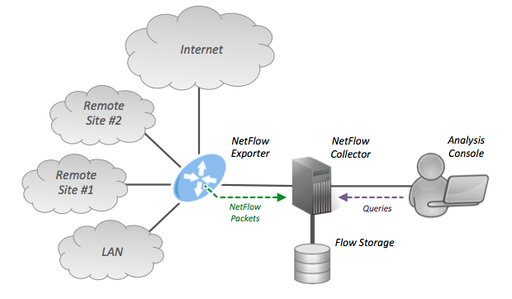
\includegraphics[width=1\textwidth]{Figures/netflow}
\decoRule
\caption[Netflow]{Netflow. \cite{netflowExample}}
\label{fig:netflow}
\end{figure}

\section{Attributes of a flow}
\label{flowattributes}
The following attributes are available within a flow:
\begin{itemize}
\item Source IP
\item Destination IP
\item Protocol name
\item Source port
\item Destination port
\item Starting time of the flow
\item Duration of the flow
\item Amount of packets in the flow
\item Amount of bytes in the flow
\end{itemize}
These attributes are most commonly available within a flow. However there are different standards for a flow. Some contain less information, some contain more information. Should a flow exporter be implemented, some additional features can be generated from packet data. 
\begin{itemize}
\item Amount of TCP SYN within the flow
\item Source and Destination Type of Service
\item TCP flags set
\end{itemize}

\noindent These extra attributes can be very usefull when trying to determine what is normal and abnormal behaviour. \\
\\
\noindent The \textbf{source IP} is the IP address of the device or network that started the flow. The \textbf{destination IP} is the IP address of the device or network that the sender connected to. The IP address can be either an IPv4 or an IPv6 address. If the flows were gathered and created on a host computer, the IP address field can be a MAC address instead of an actual IP address. These type of flows are generated by newer flow exporters.\\
\\
The \textbf{source port} is the port from which the flow originates. The \textbf{destination port} is the port to which the flow connects to. \\
\\
The \textbf{protocol name} is the name of the protocol that is used for the flow. Each flow uses only one protocol. Some flow exporters might provide the protocol is numerical form, others in ASCII format. The numerical form is used mostly by flow exporters that only allow explicit IP traffic. Other flow exporters also contain non-IP traffic such as ICMP messages. \\
\\
Flow attributes such as the \textbf{amount of packets} and the \textbf{amount of bytes} are self-explanatory. They are usefull to know for example whether the flow contains many packets which each contain almost no payload, or whether the flow contains one gigantic packet. \\
\\
The \textbf{starting time} is the time when the flow is started. This is saved in unix time. The \textbf{duration of the flow} is the time between the start and end of a connection. When the flow is a TCP connection, the start and end times are defined. These are the moments that a SYN is sent and a FIN ACK is received. However, should the flow be an UDP flow for example, there is no clear end. The flow terminates itself after a timeout. 

\section{Using IP flows}
In order to be able to use IP flows, data has to be extracted from the flows. In general, the different attributes from a flow are already useful. However it could also be interesting to extract other information from the flows. 

\subsection{Country of origin}
The country of origin is something that can be extracted from flow information. The source and the destination IP can be given to an IP API which gives back information about the physical location of the IP address. Also the region, city name and ISP can be extracted. An example of such a query can be seen in Figure~\ref{fig:ipapi}. This API is just one example of the available API's on the web. \cite{ipAPI}

\begin{figure}[H]
\centering
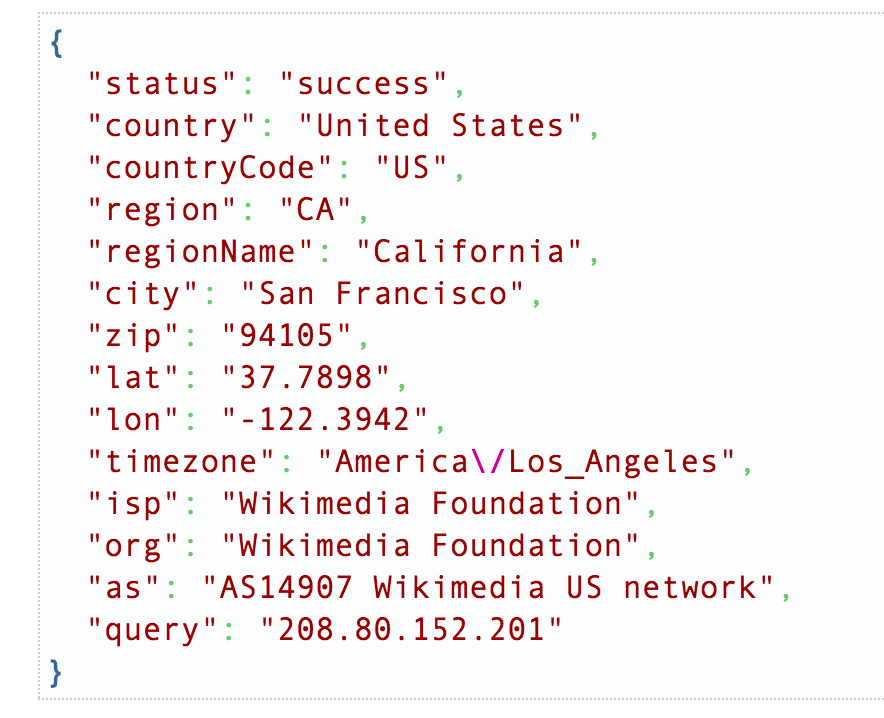
\includegraphics[width=0.6\textwidth]{Figures/ip-api}
\decoRule
\caption[IP API JSON format]{IP API JSON format. \cite{ipAPI}}
\label{fig:ipapi}
\end{figure}

\subsection{Time}
\label{timeflow}
The starting time can also be manipulated. From the unix starting time, information such as the year, month, day, weekday, hours and so on can be found. This information makes it easier to categorize network traffic and allows certain patterns to be seen. For example, it might be that certain types of web traffic only happen at a certain weekday.



